\subsection{Course log}
The sequence diagram in figure \ref{3img:[sequence]course_log} shows the
details of how the information system handles the procedure needed to
update the log of a course.

This process is useful in order to permit to the people who following the
course to be updated with the last topic treated, and from the other side,
to check that the lecturers covers all the topics prefixed.

The infrastructures used to accomplish this process are the accounting
service for authentication and the Administrative server, in which store
the entry of the log.

\begin{figure}[H]
\begin{centering}
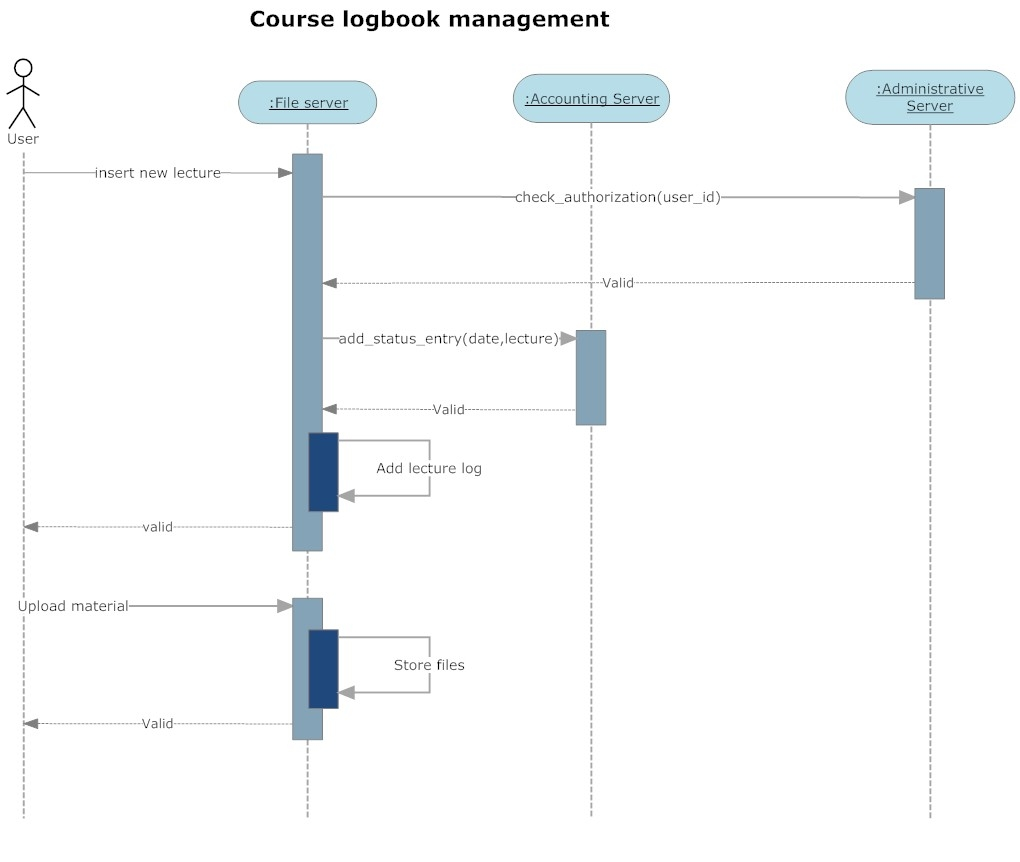
\includegraphics[scale=0.42]{assign3/sdraw/imgs/course_log.jpg}
\caption{Course log sequence diagram.}
\label{3img:[sequence]course_log}
\end{centering}
\end{figure}

\subsection{Certification}
The main aim of the course and the relative exams is to deliver the
needed certifications. The information system handles this process
following the sequence diagram in figure
\ref{3img:[sequence]certification}.

The service provided by the system is to produce a document which attest
the certification for the people who pass the exam.

In order to accomplish this task the system has to gain access to the
customers information, their exam outcomes, and to the certification
details.
 
\begin{figure}[H]
\begin{centering}
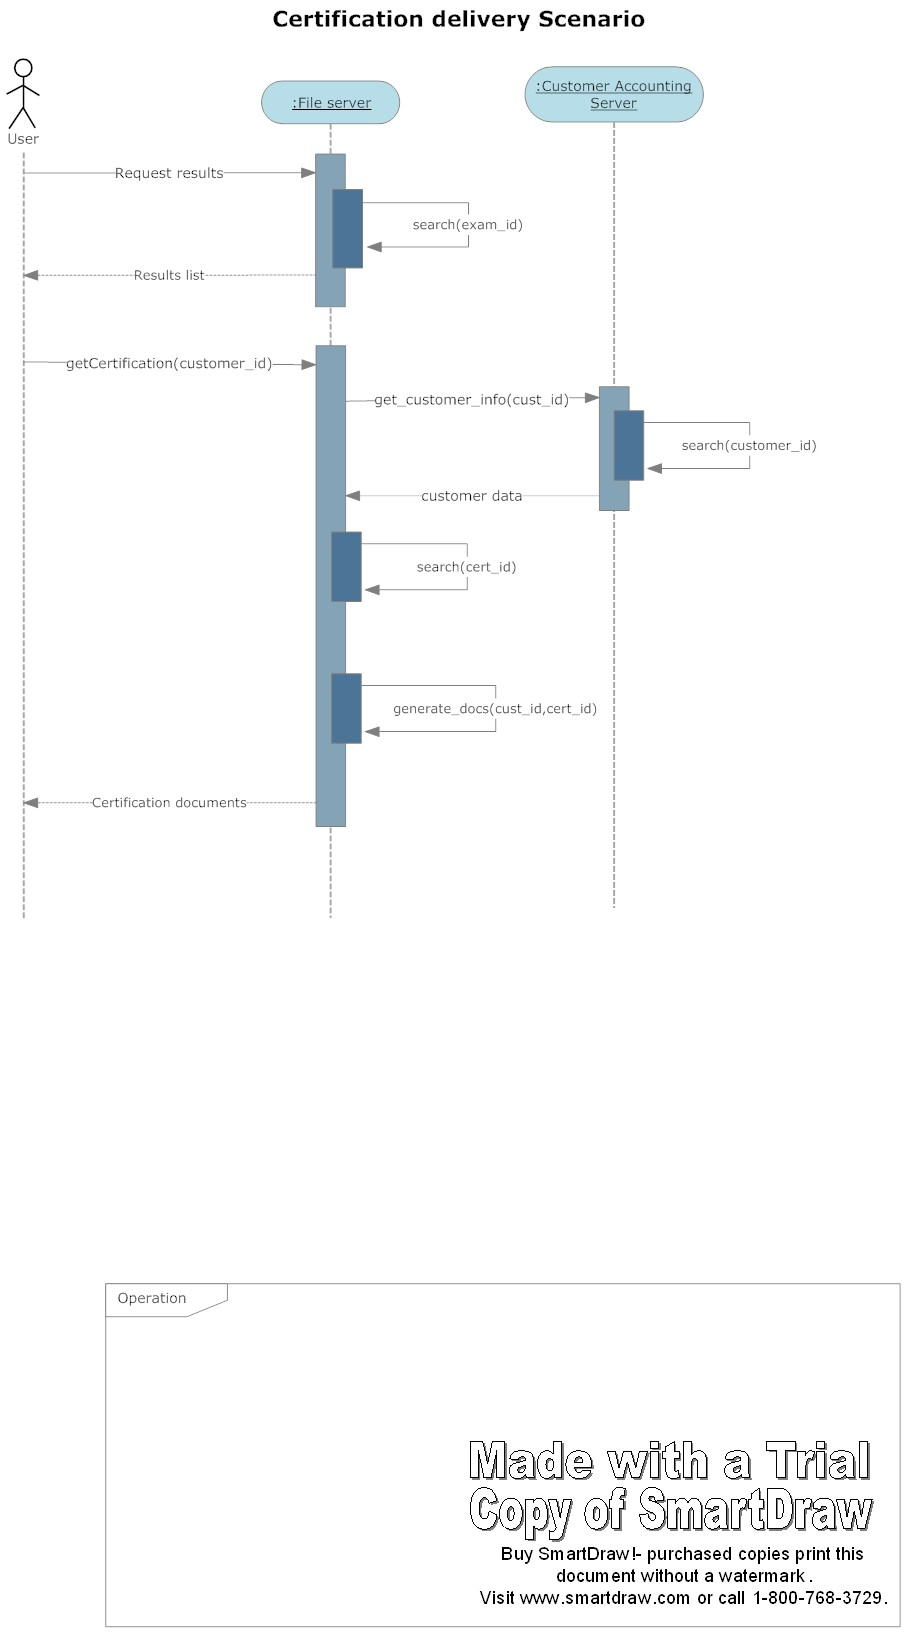
\includegraphics[scale=0.45]{assign3/sdraw/imgs/certification.jpg}
\caption{Certification sequence diagram.}
\label{3img:[sequence]certification}
\end{centering}
\end{figure}
